\documentclass[11pt]{article}

\usepackage[a4paper,margin=2.5cm]{geometry}
\usepackage[spanish]{babel}
\usepackage[utf8]{inputenc}
\usepackage[T1]{fontenc}
\usepackage{graphicx}
\usepackage{booktabs}
\usepackage{longtable}
\usepackage{array}
\usepackage{hyperref}
\usepackage{amsmath}
\usepackage{titlesec}
\usepackage{caption}
\usepackage{enumitem}
\usepackage{xcolor}
\usepackage{fancyhdr}
\usepackage{float}

\graphicspath{{images/}}

\definecolor{uanlblue}{HTML}{1164AD}
\definecolor{uanlred}{HTML}{EF796D}

\hypersetup{
    colorlinks=true,
    linkcolor=uanlblue,
    urlcolor=uanlblue,
    citecolor=uanlblue,
    pdftitle={Detección de Clientes Anómalos en E-commerce},
    pdfauthor={Andrea Linette Mezquita Gómez, Carlos Enrique Cepeda Fuentes, Miguel Alejandro Blanco Ríos}
}

\titleformat{\section}{\normalfont\Large\bfseries\color{uanlblue}}{\thesection}{1em}{}
\titleformat{\subsection}{\normalfont\large\bfseries}{\thesubsection}{1em}{}
\titleformat{\subsubsection}{\normalfont\normalsize\bfseries}{\thesubsubsection}{1em}{}

\pagestyle{fancy}
\fancyhf{}
\fancyfoot[C]{\thepage}
\renewcommand{\headrulewidth}{0pt}

\newcolumntype{L}[1]{>{\raggedright\arraybackslash}p{#1}}

\title{\textbf{Detección de Clientes Anómalos en E-commerce}\\[0.3cm]
\large Producto Integrador de Aprendizaje (PIA)}
\author{
Andrea Linette Mezquita Gómez \\
Carlos Enrique Cepeda Fuentes \\
Miguel Alejandro Blanco Ríos
}
\date{Fecha de entrega: Jueves 13 de agosto de 2026}

\begin{document}

% ── PORTADA ──────────────────────────────────────────────────
\begin{titlepage}
  \noindent
  
\includegraphics[height=2cm]{logo_uanl.jpeg}%
  \hfill%
  
\includegraphics[height=2cm]{logo_fcfm.jpeg}
  \centering
  \vspace{1cm}

  {\large\textbf{Universidad Autónoma de Nuevo León}}\\[0.4em]
  {\large Facultad de Ciencias Físico Matemáticas}\\[0.4em]
  {\large Maestría en Ciencia de Datos}

  \vspace{2.5cm}

  {\LARGE\textbf{Detección de Clientes Anómalos en E-commerce}}\\[0.6em]
  {\Large Producto Integrador de Aprendizaje (PIA)}\\[0.3em]
  {\large Aprendizaje Automático}

  \vspace{2.5cm}

  \begin{tabular}{rl}
    \textbf{Alumnos:}          & Andrea Linette Mezquita Gómez \\
                                & Carlos Enrique Cepeda Fuentes \\
                                & Miguel Alejandro Blanco Ríos \\[0.5em]
    \textbf{Profesor:}         & Irving Daniel Estrada López \\[0.5em]
    \textbf{Fecha de entrega:} & Jueves 13 de agosto de 2026 \\
  \end{tabular}

  \vfill
\end{titlepage}

\tableofcontents
\newpage

\section*{Definición del Proyecto}
\addcontentsline{toc}{section}{Definición del Proyecto}

En un negocio de comercio electrónico, la gran mayoría de los clientes siguen patrones de compra
relativamente homogéneos: compran con cierta frecuencia, gastan montos similares y devuelven una
fracción pequeña de sus pedidos. Sin embargo, dentro de cualquier base de clientes existen casos atípicos
(compradores con comportamientos que se desvían sustancialmente del resto), cuya identificación
temprana tiene valor de negocio directo: pueden representar clientes de alto valor a retener, cuentas con
actividad fraudulenta, errores de captura de datos, o segmentos emergentes que ameritan una estrategia
comercial distinta.

Este proyecto aborda dicha necesidad como un problema de detección de anomalías (\textit{anomaly detection})
no supervisada: no se cuenta con una variable objetivo que indique de antemano qué clientes son
``anómalos'', por lo que la tarea consiste en aprender la estructura general del comportamiento de compra
y señalar, de forma automática, a los clientes que se apartan de dicha estructura.

\subsection*{Alcance y metodología}

El proyecto se desarrolló siguiendo un flujo de trabajo inspirado en prácticas de MLOps, con el fin de que
el pipeline sea reproducible y no dependa únicamente de la ejecución manual de un notebook monolítico.
El repositorio del proyecto separa el flujo en etapas independientes y persistidas en disco, cada una con
su propio notebook de exploración y su módulo equivalente en Python:

\begin{longtable}{L{3.2cm}L{5cm}L{6cm}}
\toprule
\textbf{Etapa} & \textbf{Entrada} & \textbf{Salida} \\
\midrule
\endhead
Carga de datos & \texttt{data/raw/*.xlsx} & \texttt{data/processed/customer\_features.csv} \\
Exploración de datos (EDA) & \texttt{customer\_features.csv} & (solo análisis) \\
Preprocesamiento & \texttt{customer\_features.csv} & \texttt{customer\_features\_model.csv} \\
Entrenamiento & \texttt{customer\_features\_model.csv} & \texttt{models/isolation\_forest.joblib}, \texttt{best\_params.json} \\
Validación & \texttt{customer\_features\_model.csv}, \texttt{model\_predictions.csv} & (solo evaluación) \\
\bottomrule
\end{longtable}

Esta separación permite ejecutar cada etapa de forma independiente, versionar los artefactos generados
(dataset procesado, modelo entrenado, hiperparámetros óptimos) y reutilizar el modelo de Isolation
Forest sin reentrenar. DBSCAN, al ser un algoritmo transductivo (no expone un método \texttt{predict()}
independiente sobre datos nuevos), únicamente persiste sus etiquetas sobre el conjunto de
entrenamiento.

\subsection*{Justificación de los modelos seleccionados}

Se seleccionaron dos modelos no supervisados vistos en el curso, de naturaleza deliberadamente distinta,
para poder contrastar dos filosofías de detección de anomalías:

\begin{itemize}
    \item \textbf{DBSCAN (Density-Based Spatial Clustering of Applications with Noise):} un algoritmo de
    clustering basado en densidad cuyo subproducto natural (los puntos etiquetados como ``ruido'')
    se puede reinterpretar como el conjunto de anomalías. Se eligió porque permite evaluar si las
    anomalías del dataset corresponden a zonas de baja densidad bien definidas.
    \item \textbf{Isolation Forest:} un modelo de ensamble diseñado específicamente para detección de anomalías,
    que no requiere una noción de distancia ni de densidad, sino de aislamiento estructural. Se eligió
    como contraparte porque ataca el mismo problema desde un principio matemático completamente
    distinto, lo que permite una comparación metodológicamente rica.
\end{itemize}

\section*{Datos}
\addcontentsline{toc}{section}{Datos}

\subsection*{Fuente de datos}

El proyecto utiliza dos dataset públicos: ``Online Retail'' y su extensión ``Online Retail II'', disponibles en el
UCI Machine Learning Repository. Ambos conjuntos contienen el registro transaccional (a nivel línea de
factura) de una tienda de e-commerce con sede en el Reino Unido, entre los años 2009 y 2011, incluyendo
el identificador de factura, código y descripción del producto, cantidad, precio unitario, fecha de la
transacción, identificador de cliente y país de envío.

Ambos archivos se cargan de forma independiente y se combinan en un único dataset transaccional.

\subsection*{Limpieza y construcción del dataset}

El dataset transaccional crudo no es directamente utilizable por los modelos de detección de anomalías,
ya que la unidad de análisis del proyecto es el cliente, no la línea de factura. El procesamiento aplicado
fue:

\begin{itemize}
    \item Eliminación de registros sin \texttt{CustomerID} (transacciones no atribuibles a un cliente identificado).
    \item Exclusión de clientes cuyas compras corresponden a productos de prueba interna (\texttt{StockCode} que contiene ``test'').
    \item Separación de las transacciones en compras (\texttt{Quantity} $\geq$ 0) y devoluciones (\texttt{Quantity} $<$ 0), para poder calcular una tasa de devolución por cliente.
    \item Cálculo de la variable \texttt{Sales = Quantity} $\times$ \texttt{UnitPrice} como base para las métricas monetarias agregadas.
    \item Agregación de todas las transacciones a nivel \texttt{CustomerID}, resultando en un dataset de 5,876 clientes y 10 variables.
\end{itemize}

\subsubsection*{Variables construidas por cliente}

\begin{longtable}{L{3.2cm}L{3.2cm}L{8.5cm}}
\toprule
\textbf{Variable} & \textbf{Tipo} & \textbf{Descripción} \\
\midrule
\endhead
Pais Principal & Categórica nominal & País donde el cliente realizó la mayoría de sus compras \\
Paises Distintos & Numérica (conteo) & Cantidad de países distintos desde los que ha comprado \\
Permanencia & Continua & Días transcurridos entre la primera y la última compra \\
Compras & Continua (conteo) & Número de órdenes distintas realizadas \\
Canasta\_Prom & Continua & Unidades promedio por compra \\
Ticket\_Prom & Continua & Monto promedio gastado por compra (\texttt{Sales / Compras}) \\
Precio\_Prom & Continua & Precio promedio ponderado por unidades vendidas (\texttt{Sales / Quantity}), no el promedio simple de precios unitarios por línea de producto \\
Precio\_Max & Continua & Precio unitario más alto entre los productos comprados por el cliente \\
Productos Distintos & Continua (conteo) & Variedad de productos distintos comprados \\
Pct\_Devoluciones & Continua (proporción) & Proporción de órdenes que fueron devueltas \\
\bottomrule
\end{longtable}

\subsection*{Análisis exploratorio de datos (EDA)}

\subsubsection*{Estadísticas descriptivas}

Las estadísticas descriptivas muestran una dispersión considerable en la mayoría de las variables. Por
ejemplo, el cliente mediano realiza 3 compras y permanece activo 221.5 días, pero existen clientes con
hasta 398 compras y hasta 739 días de permanencia. De forma similar, el precio promedio por producto
tiene una mediana de \$1.83, pero un máximo de \$10,953, una diferencia de varios órdenes de magnitud
que ya anticipa la presencia de outliers extremos y una fuerte asimetría positiva en casi todas las variables
monetarias.

El porcentaje de devoluciones tiene una mediana de 0\% (la mitad de los clientes no devuelve nada) pero
un máximo de 400\% (clientes cuyas devoluciones superan, en unidades, a sus compras del mismo
periodo).

\subsubsection*{Distribución y correlación de variables numéricas}

Dado que las variables de conteo y monto (Compras, Canasta\_Prom, Ticket\_Prom, Precio\_Prom,
Precio\_Max, Productos Distintos) presentan histogramas fuertemente sesgados a la derecha, se aplicó
una transformación logarítmica (\texttt{log1p}) antes de examinar su correlación, con el fin de que la matriz de
dispersión y los coeficientes de Pearson no estuvieran dominados por unos cuantos valores extremos.

\begin{figure}[H]
    \centering
    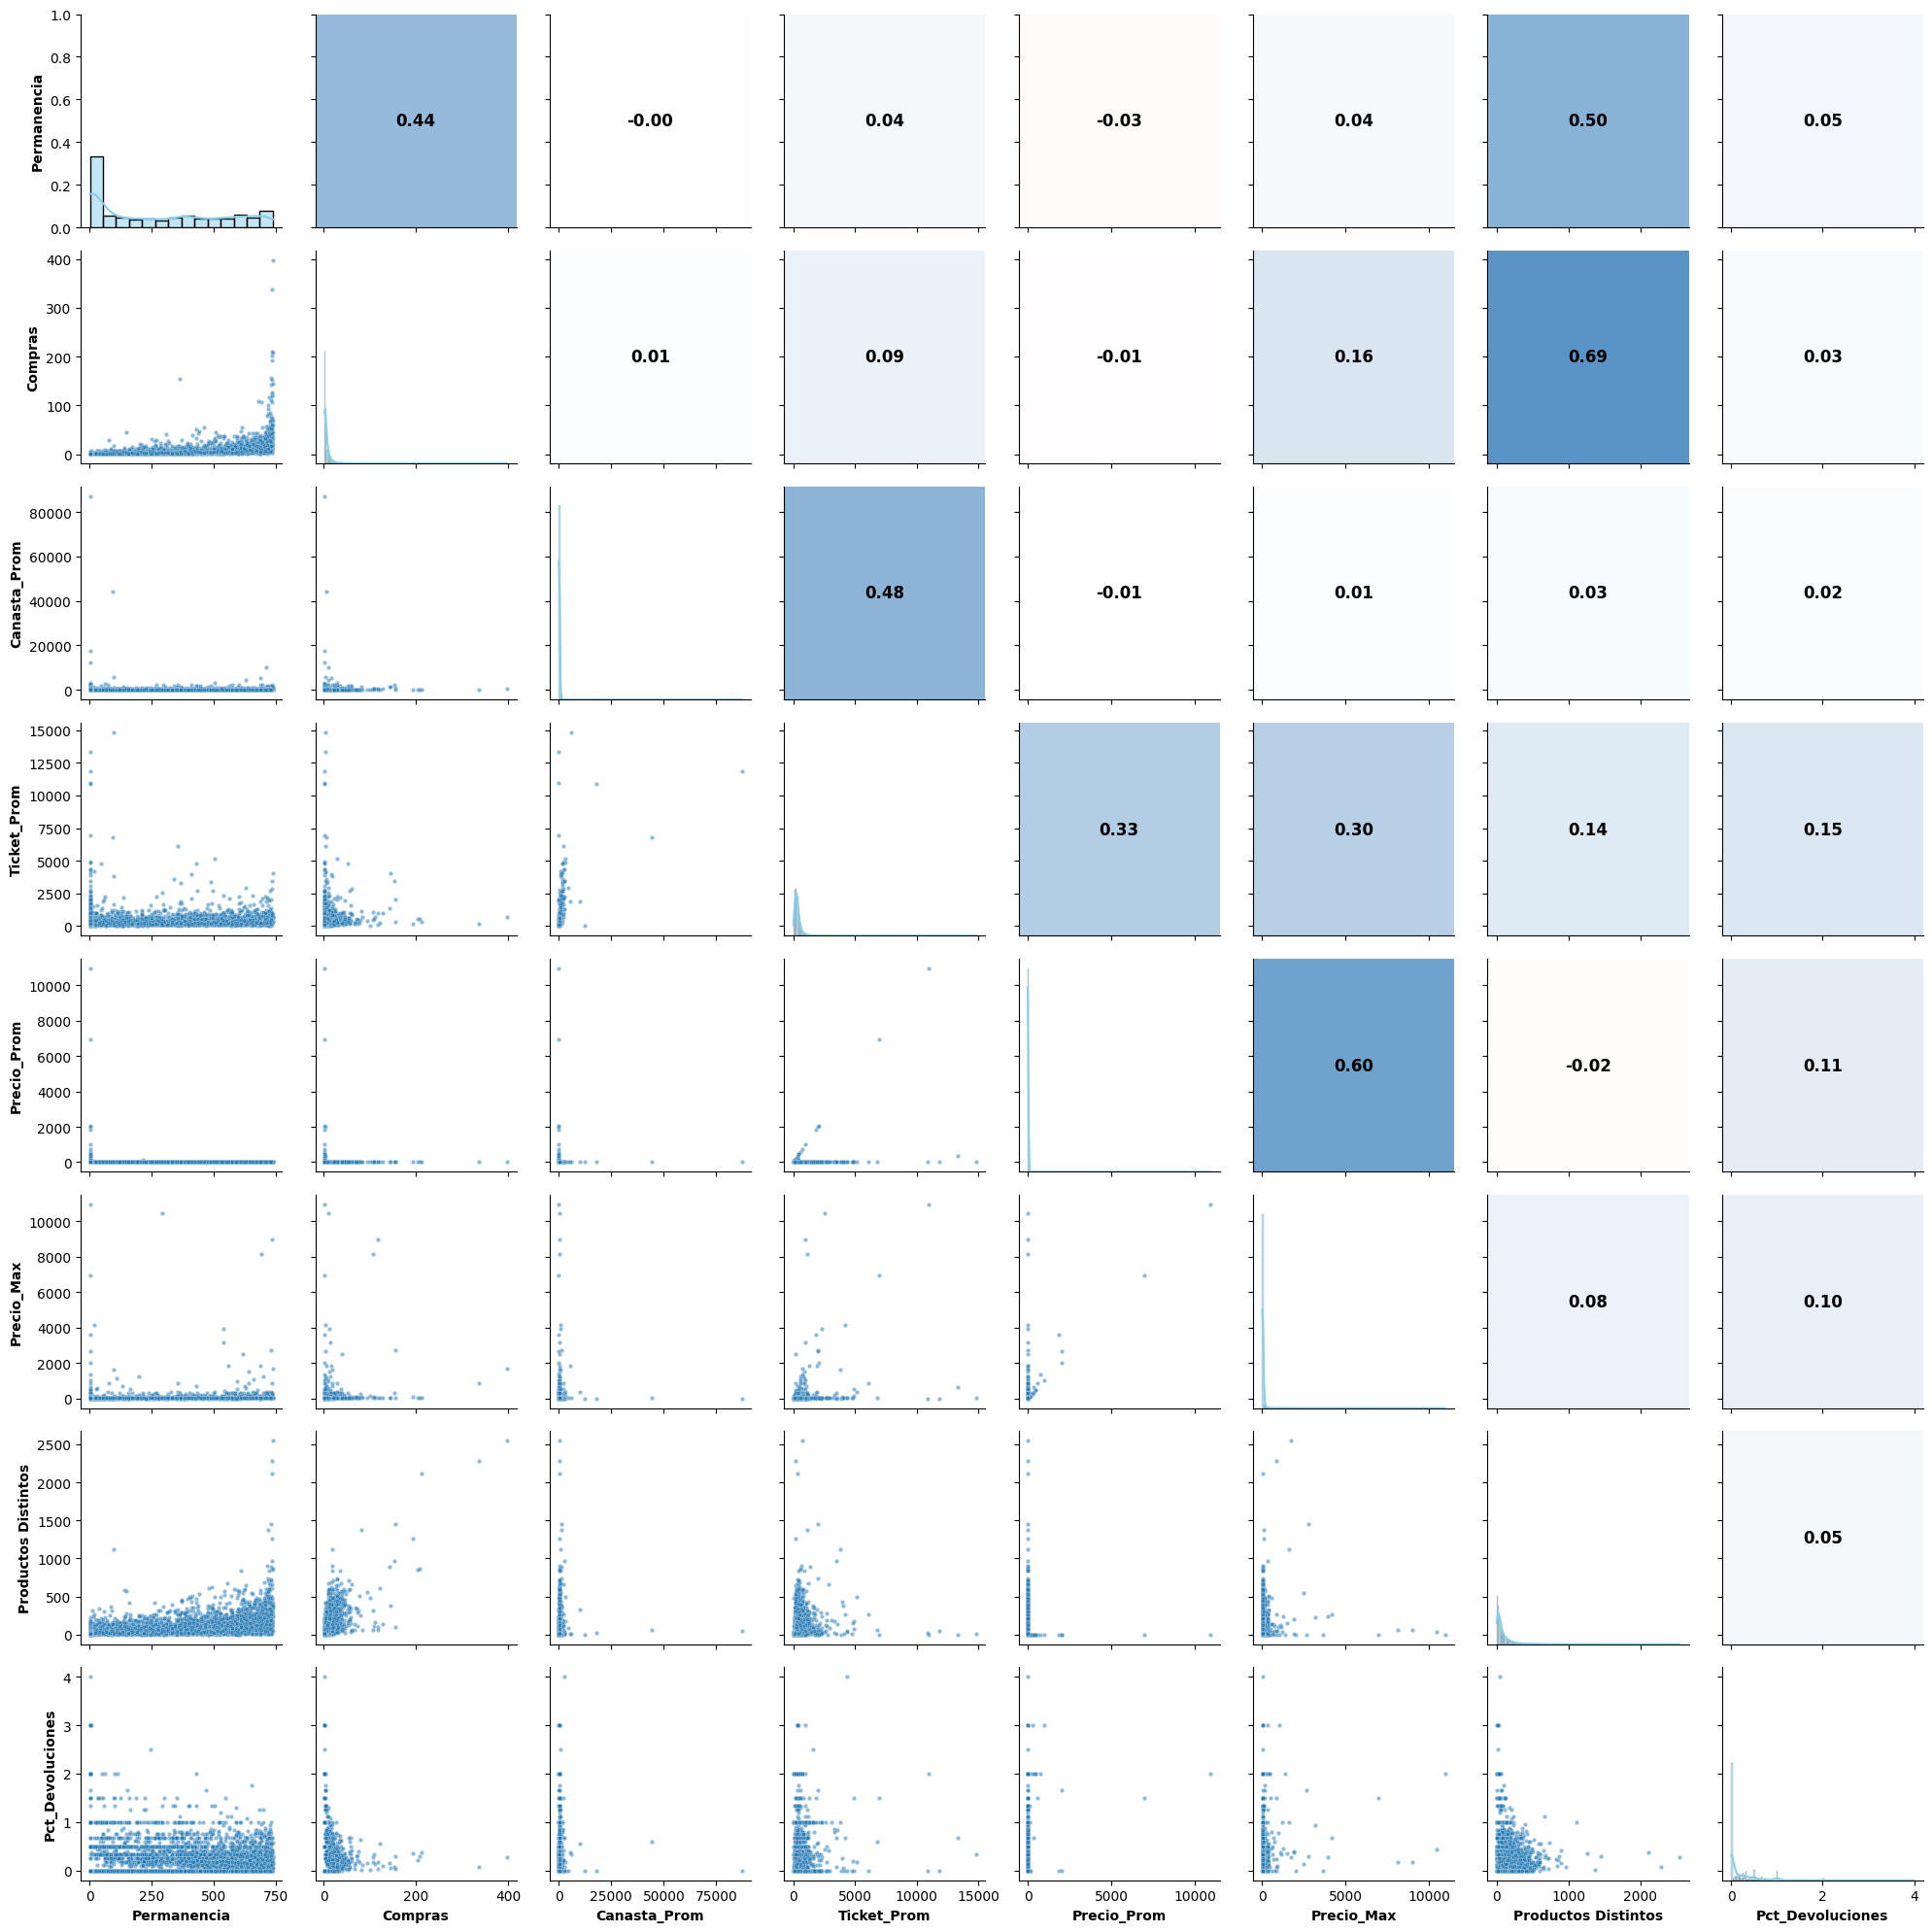
\includegraphics[width=0.85\textwidth]{fig01_correlacion_original.png}
    \caption{Matriz de dispersión y correlación de Pearson de las variables numéricas originales (sin transformar).}
    \label{fig:corr-original}
\end{figure}

\begin{figure}[H]
    \centering
    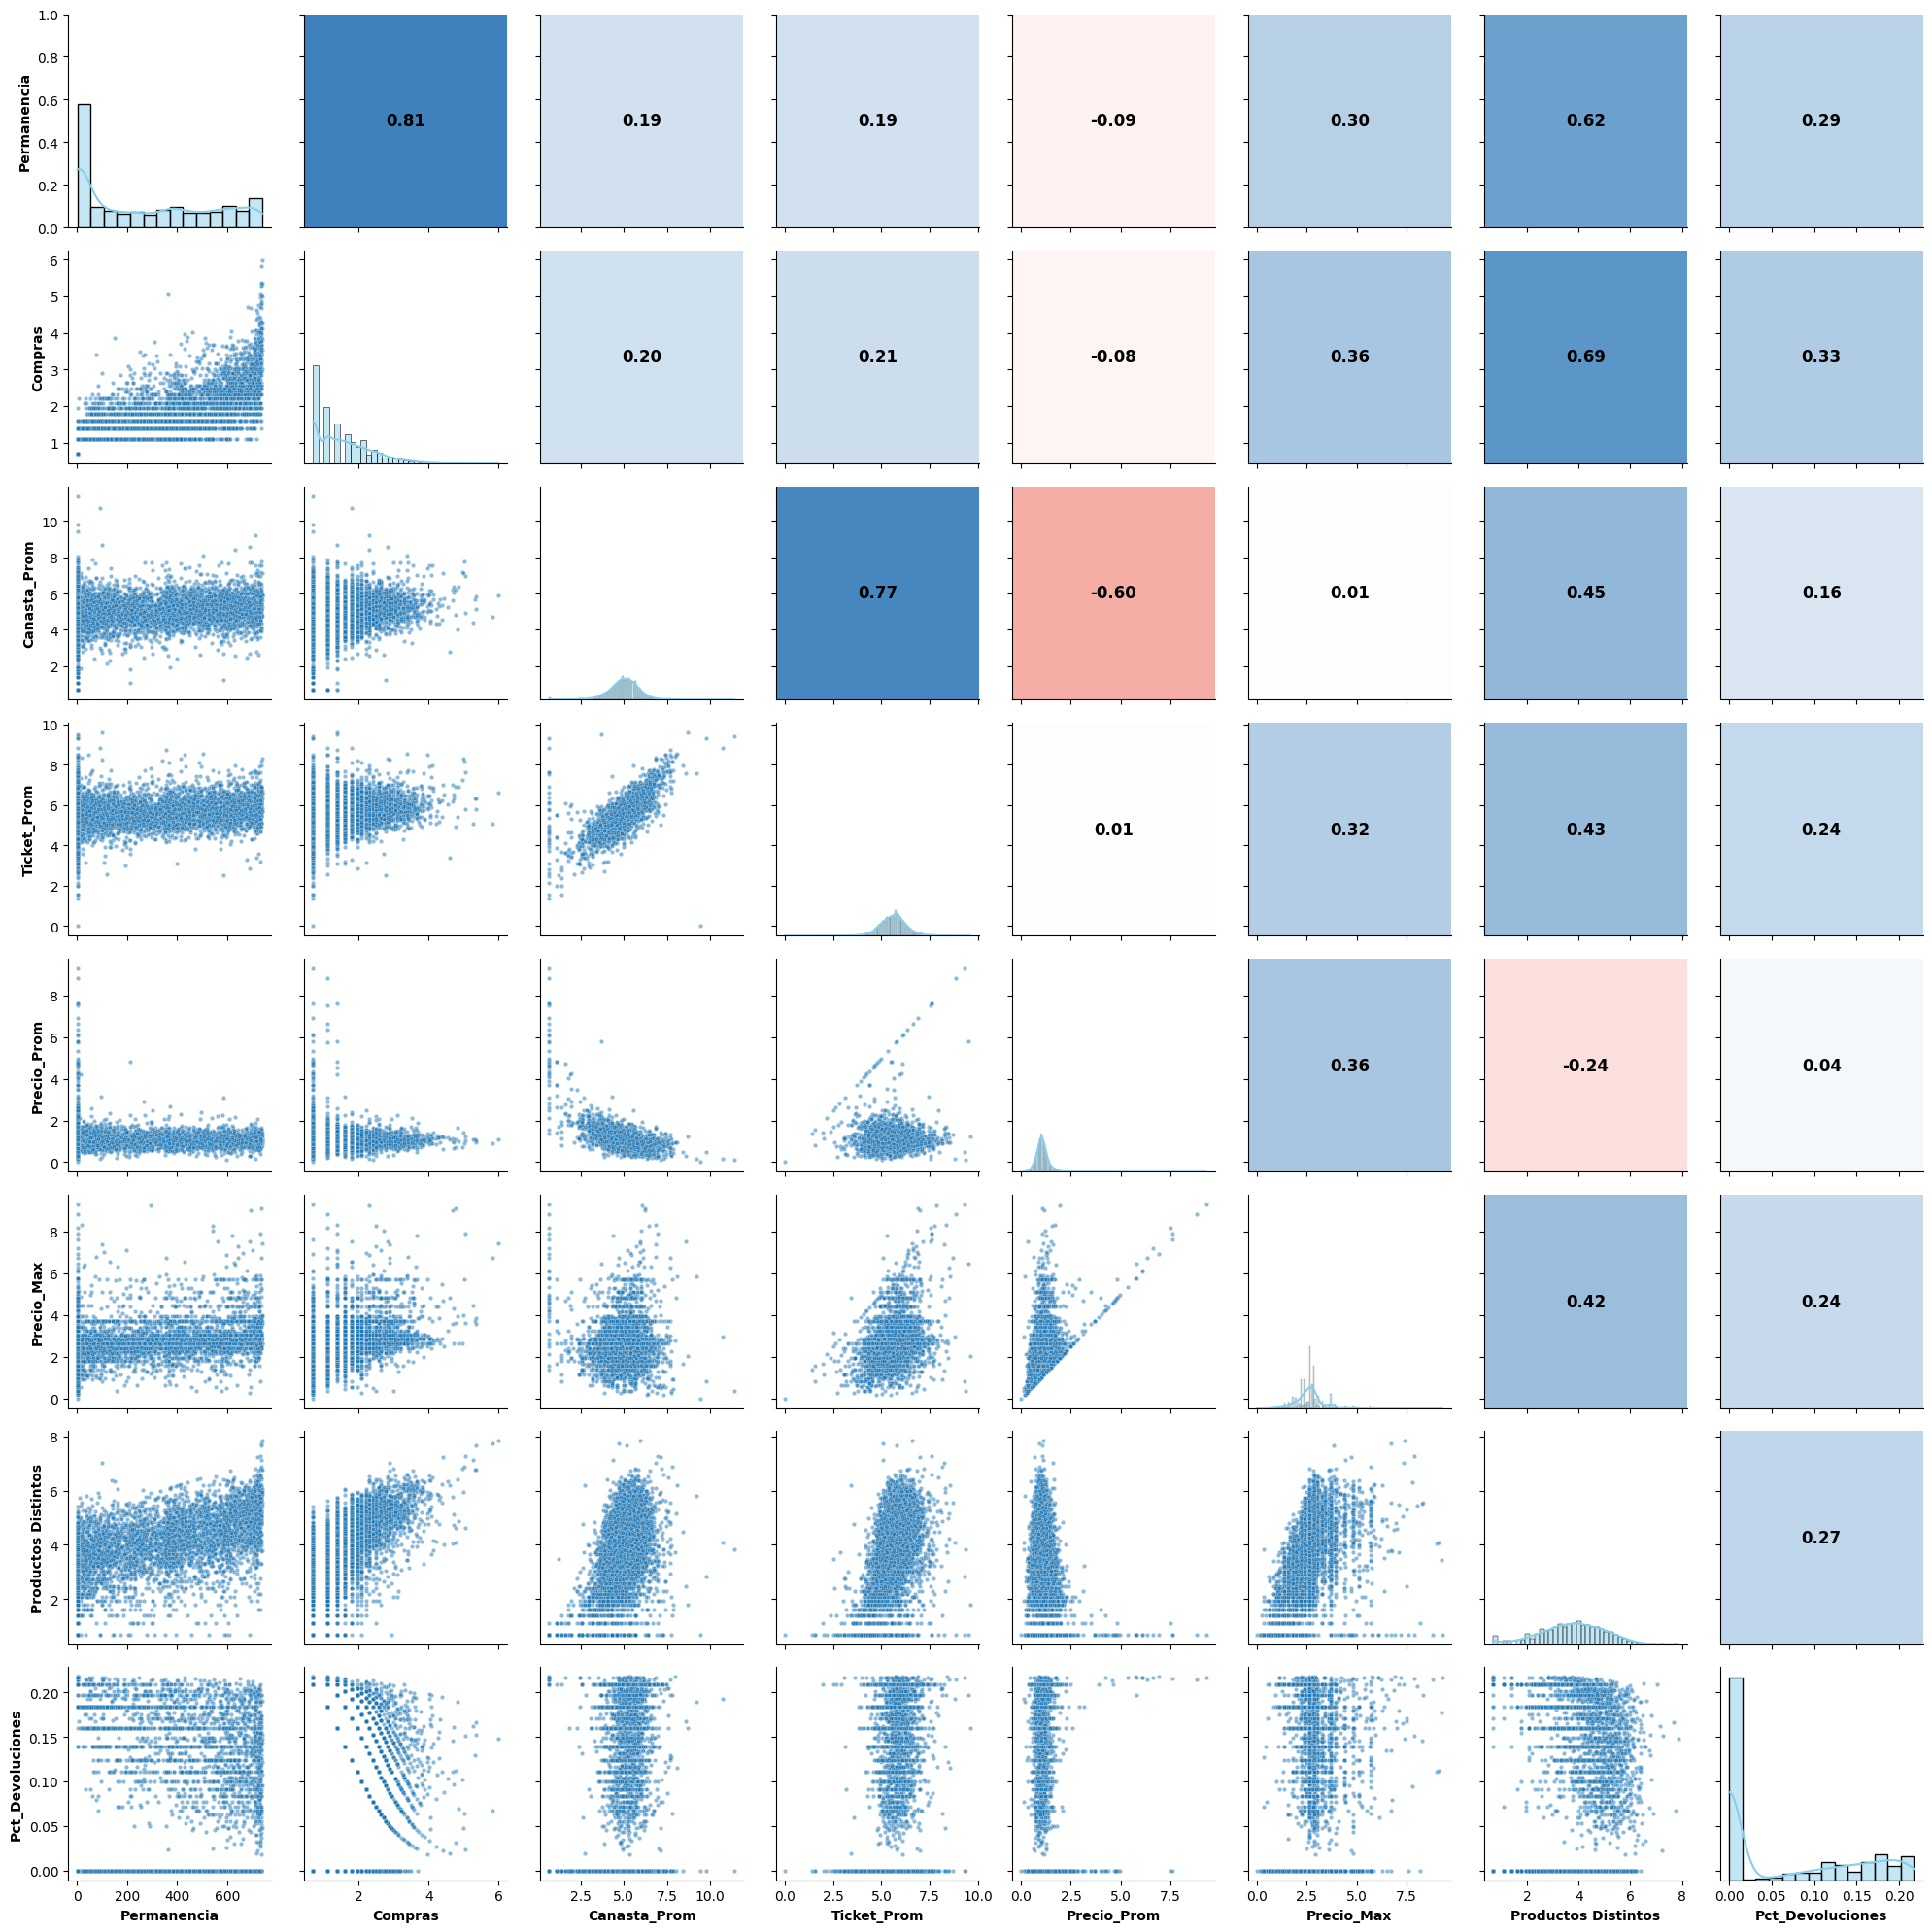
\includegraphics[width=0.85\textwidth]{fig02_correlacion_log1p.png}
    \caption{Matriz de dispersión y correlación de Pearson tras la transformación log1p. Las distribuciones de la diagonal se aproximan más a la normal.}
    \label{fig:corr-log1p}
\end{figure}

Los patrones de correlación más relevantes, ya con la transformación aplicada, son:

\begin{itemize}
    \item \textbf{Compras $\times$ Permanencia:} correlación positiva alta (+0.81). A mayor tiempo como cliente, mayor cantidad de compras realizadas.
    \item \textbf{Compras $\times$ Productos Distintos:} correlación positiva alta (+0.69). A mayor número de compras, mayor variedad de productos adquiridos.
    \item \textbf{Canasta\_Prom $\times$ Ticket\_Prom:} correlación positiva alta (+0.77). A mayor cantidad de unidades por compra, mayor el valor monetario promedio de la compra.
    \item \textbf{Canasta\_Prom $\times$ Precio\_Prom:} correlación negativa alta (-0.60). A menor precio unitario, mayor la cantidad de unidades adquiridas.
\end{itemize}

\subsubsection*{Variables categóricas}

\begin{figure}[H]
    \centering
    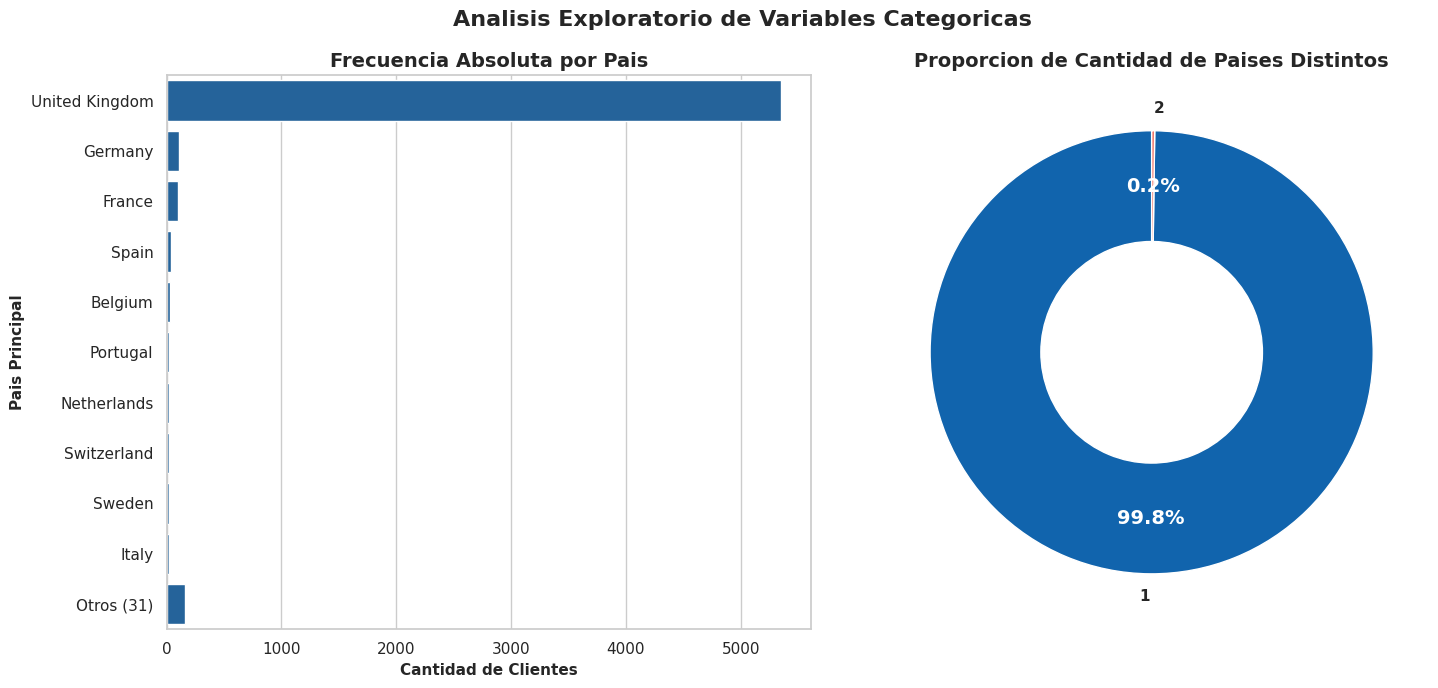
\includegraphics[width=0.85\textwidth]{fig03_categoricas.png}
    \caption{Distribución de Pais Principal y Paises Distintos.}
    \label{fig:categoricas}
\end{figure}

El 91\% de los clientes concentra la mayoría de sus compras en el Reino Unido; el 9\% restante se distribuye
entre otros 40 países. Asimismo, el 99.8\% de los clientes compra exclusivamente desde un solo país, y
únicamente una fracción marginal lo hace desde dos. Esta alta concentración es la que justificó, más
adelante, resumir ambas variables categóricas en dos binarias en lugar de aplicar one-hot encoding
directo sobre 41 categorías.

\subsubsection*{Detección visual de valores atípicos}

\begin{figure}[H]
    \centering
    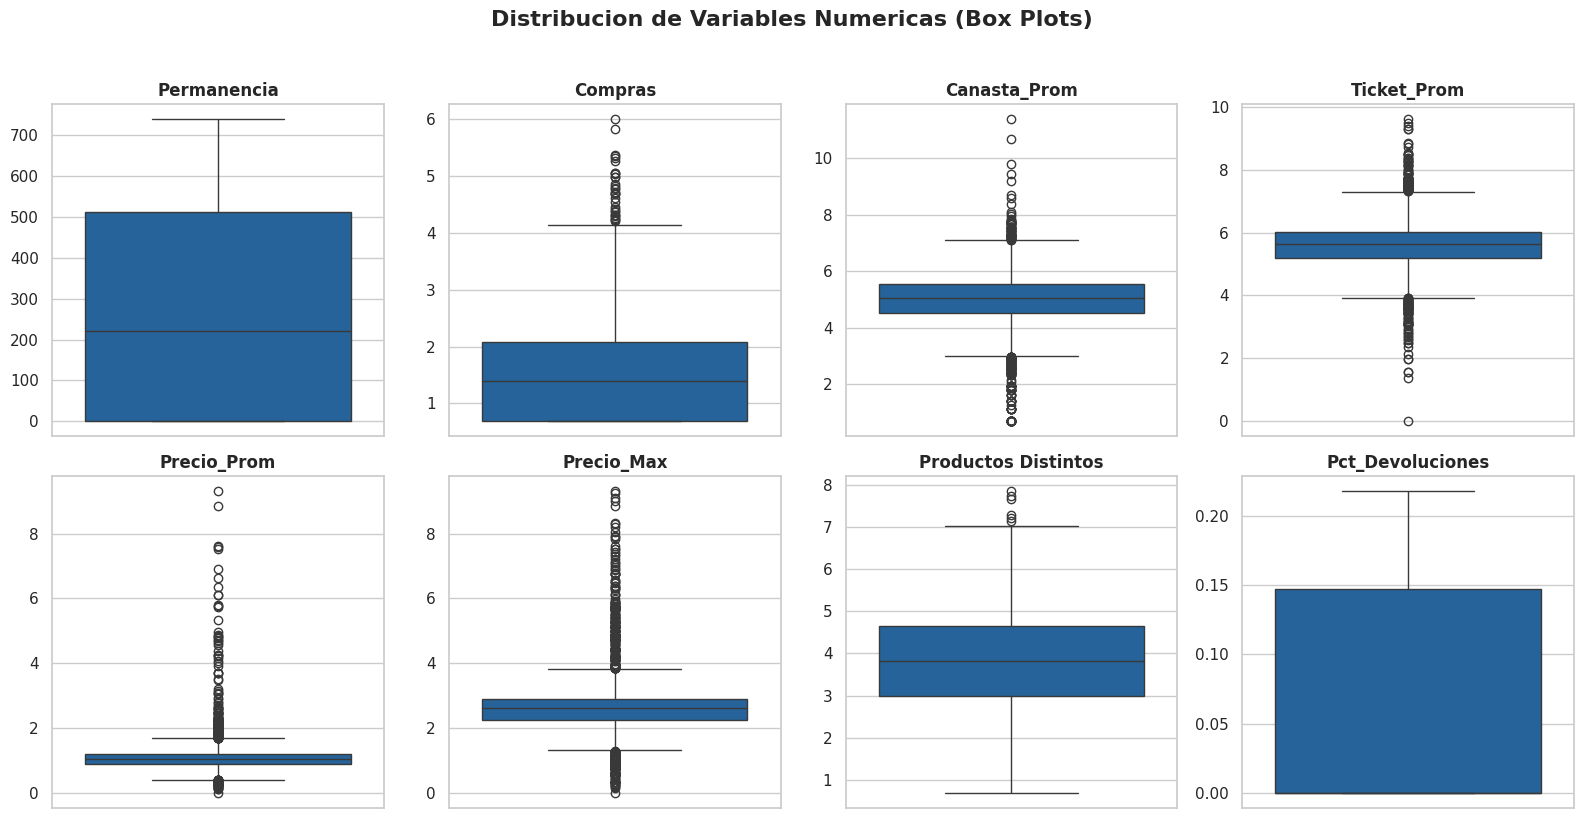
\includegraphics[width=0.85\textwidth]{fig04_boxplots.png}
    \caption{Diagramas de caja (boxplots) de las variables numéricas continuas.}
    \label{fig:boxplots-eda}
\end{figure}

Los boxplots confirman lo observado en las estadísticas descriptivas: Compras, Canasta\_Prom,
Ticket\_Prom, Precio\_Prom y Precio\_Max muestran numerosos outliers positivos (y en algunos casos
negativos), es decir, clientes cuyo comportamiento de compra se aleja sustancialmente de la mayoría.
Permanencia, en cambio, se mantiene acotada entre 0 y aproximadamente 700 días sin outliers extremos.

Estos valores atípicos son, precisamente, el fenómeno que los modelos de detección de anomalías buscan
capturar de forma sistemática, por lo que, a diferencia de un pipeline de modelado predictivo tradicional,
\textbf{no se eliminan ni se recortan en esta etapa}.

\section*{Preprocesamiento de Datos}
\addcontentsline{toc}{section}{Preprocesamiento de Datos}

El preprocesamiento tiene como objetivo dejar todas las variables en una representación numérica y en
una escala comparable, de forma que ni DBSCAN (basado en distancia euclidiana) ni Isolation Forest
(basado en cortes aleatorios por variable) se vean sesgados por diferencias de magnitud entre variables.

\subsection*{Transformación logarítmica}

Como se explicó en la sección de EDA, las variables de conteo y monto presentan una distribución sesgada
a la derecha, típica de fenómenos multiplicativos (gasto, cantidad de unidades). Se aplicó la
transformación:

\begin{equation}
y = \log(1 + x)
\end{equation}

conocida como \texttt{log1p}, a las variables Compras, Canasta\_Prom, Ticket\_Prom, Precio\_Prom, Precio\_Max y
Productos Distintos. El uso de $\log(1+x)$ en vez de $\log(x)$ evita la indeterminación matemática cuando $x = 0$
(frecuente en variables de conteo), y comprime la cola derecha de la distribución sin alterar el orden
relativo de las observaciones, ya que el logaritmo es una función estrictamente creciente.

Es importante señalar el trade-off que implica esta decisión: dado que el objetivo del proyecto es detectar
valores extremos, comprimir la escala de las variables con mayor sesgo también atenúa parcialmente la
separación entre observaciones normales y extremas. Se optó por aplicar la transformación de cualquier
forma porque, sin ella, los modelos basados en distancia (DBSCAN en particular) tienden a ser dominados
casi por completo por un puñado de valores extremos, impidiendo distinguir cualquier estructura de
densidad en el resto del espacio de variables.

\subsection*{Codificación de variables categóricas}

Dado que Pais Principal tiene 41 categorías únicas y está altamente concentrada (91\% en un solo valor),
un one-hot encoding directo generaría 41 columnas dispersas que, combinadas, podrían terminar
pesando más que las 8 variables continuas originales al calcular distancias euclidianas, precisamente el
problema que se buscaba evitar. En su lugar, se resumió la información categórica relevante en dos
variables binarias con significado de negocio:

\begin{itemize}
    \item \textbf{Comprador Local} = 1 si Pais Principal es ``United Kingdom'', 0 en caso contrario.
    \item \textbf{Nomada} = 1 si Paises Distintos $>$ 1 (el cliente ha comprado desde más de un país), 0 en caso contrario.
\end{itemize}

Esta decisión sacrifica granularidad (ya no se distingue entre países específicos fuera del Reino Unido) a
cambio de mantener el espacio de variables balanceado y evitar que la codificación categórica domine el
cálculo de distancias en DBSCAN.

\subsection*{Estandarización de variables continuas}

Las 8 variables numéricas continuas (ya transformadas logarítmicamente donde aplicaba) se
estandarizaron con \texttt{StandardScaler}, que transforma cada variable a media 0 y desviación estándar 1
mediante:

\begin{equation}
z = \frac{x - \mu}{\sigma}
\end{equation}

donde $\mu$ y $\sigma$ son la media y la desviación estándar muestral de la variable. Esta estandarización es
\textbf{indispensable} para DBSCAN: al basarse en distancia euclidiana, cualquier variable en una escala numérica
mayor (por ejemplo, montos en cientos de dólares frente a conteos de 1 a 20) dominaría por completo el
cálculo de la distancia, y el parámetro \texttt{eps} dejaría de tener un significado consistente entre variables. Para
Isolation Forest la estandarización no es estrictamente necesaria pero se aplicó de igual forma para
mantener un preprocesamiento consistente entre ambos modelos y permitir una comparación justa sobre
el mismo dataset transformado.

Las dos variables binarias (Comprador Local, Nomada) se dejaron en su escala natural (0/1), sin
estandarizar, ya que estandarizar una variable binaria distorsiona su interpretación directa sin aportar
beneficio para el cálculo de distancias.

\subsection*{Dataset final para modelado}

El resultado de esta etapa es un dataset de 5,876 filas de 10 columnas (8 variables continuas
estandarizadas y 2 variables binarias), indexado por \texttt{CustomerID}, que se utiliza sin modificaciones
adicionales como entrada tanto para DBSCAN como para Isolation Forest, garantizando que ambos
modelos se evalúen sobre exactamente la misma representación del problema.

\section*{Modelos}
\addcontentsline{toc}{section}{Modelos}

Esta sección desarrolla el fundamento teórico-matemático de cada modelo, el procedimiento de
optimización de hiperparámetros empleado, y los resultados obtenidos al entrenar cada uno sobre el
dataset final.

\subsection*{DBSCAN}

DBSCAN (Density-Based Spatial Clustering of Applications with Noise) es un algoritmo de clustering no
supervisado que agrupa observaciones con base en la densidad del espacio de variables. Su definición se
apoya en dos hiperparámetros:

\begin{itemize}
    \item \textbf{eps ($\varepsilon$):} radio máximo dentro del cual se considera que dos observaciones son vecinas.
    \item \textbf{min\_samples:} número mínimo de observaciones (incluyéndose a sí misma) que deben existir dentro del radio $\varepsilon$ de un punto para que este se considere un punto núcleo (\textit{core point}).
\end{itemize}

A partir de estos parámetros, DBSCAN clasifica cada observación en una de tres categorías:

\begin{itemize}
    \item \textbf{Punto núcleo (core point):} tiene al menos \texttt{min\_samples} observaciones dentro de su $\varepsilon$-vecindario.
    \item \textbf{Punto frontera (border point):} no es núcleo, pero cae dentro del $\varepsilon$-vecindario de al menos un punto núcleo.
    \item \textbf{Punto de ruido (noise point):} no es núcleo ni frontera de ningún cluster.
\end{itemize}

Dos puntos núcleo pertenecen al mismo cluster si son \textit{density-reachable} entre sí, es decir, si existe una
cadena de puntos núcleo consecutivos, cada uno dentro del $\varepsilon$-vecindario del anterior, que los conecte.

Para efectos de detección de anomalías, la propiedad clave de DBSCAN es que no obliga a cada
observación a pertenecer a algún cluster: los puntos de ruido (aquellos ubicados en regiones de baja
densidad del espacio de variables) se etiquetan con la clase $-1$ y se reinterpretan directamente como el
conjunto de anomalías del dataset.

\subsubsection*{Optimización de hiperparámetros}

A diferencia de un modelo supervisado, DBSCAN no cuenta con una variable objetivo contra la cual medir
el error de predicción, por lo que no es posible usar validación cruzada con una métrica como el error
absoluto medio. En su lugar, se optimizaron \texttt{eps} y \texttt{min\_samples} maximizando el Silhouette Score,
calculado directamente sobre las etiquetas de cluster que produce cada combinación de hiperparámetros.

La búsqueda se realizó con Optuna, usando el muestreador Tree-structured Parzen Estimator (TPE). A
diferencia de una búsqueda de rejilla (grid search) o aleatoria pura, TPE construye de forma iterativa un
modelo probabilístico de qué regiones del espacio de hiperparámetros tienden a producir mejores
resultados, y sesga las siguientes combinaciones propuestas hacia esas regiones, resultando en una
búsqueda más eficiente en número de iteraciones.

Las combinaciones que producían un único cluster (o ningún cluster real, solo ruido) se penalizaron
devolviendo un score de $-1$, ya que el Silhouette Score no está definido cuando existe menos de dos
clusters.

\begin{table}[H]
\centering
\begin{tabular}{lll}
\toprule
\textbf{Hiperparámetro} & \textbf{Rango explorado} & \textbf{Valor óptimo} \\
\midrule
eps & [0.10, 3.00] & 0.8828 \\
min\_samples & [2, 50] & 29 \\
\bottomrule
\end{tabular}
\caption{Espacio de búsqueda e hiperparámetros óptimos de DBSCAN.}
\end{table}

El mejor valor de Silhouette Score obtenido durante la búsqueda fue de 0.0805.

\subsubsection*{Resultados del modelo}

Con los hiperparámetros óptimos, DBSCAN produjo 2 clusters reales más el grupo de ruido, marcando
2,295 clientes (39.06\% del total) como anomalía. Para visualizar el resultado en dos dimensiones, se
proyectó el dataset a 2 componentes principales mediante PCA, que retienen conjuntamente el 62.1\% de
la varianza total.

\begin{figure}[H]
    \centering
    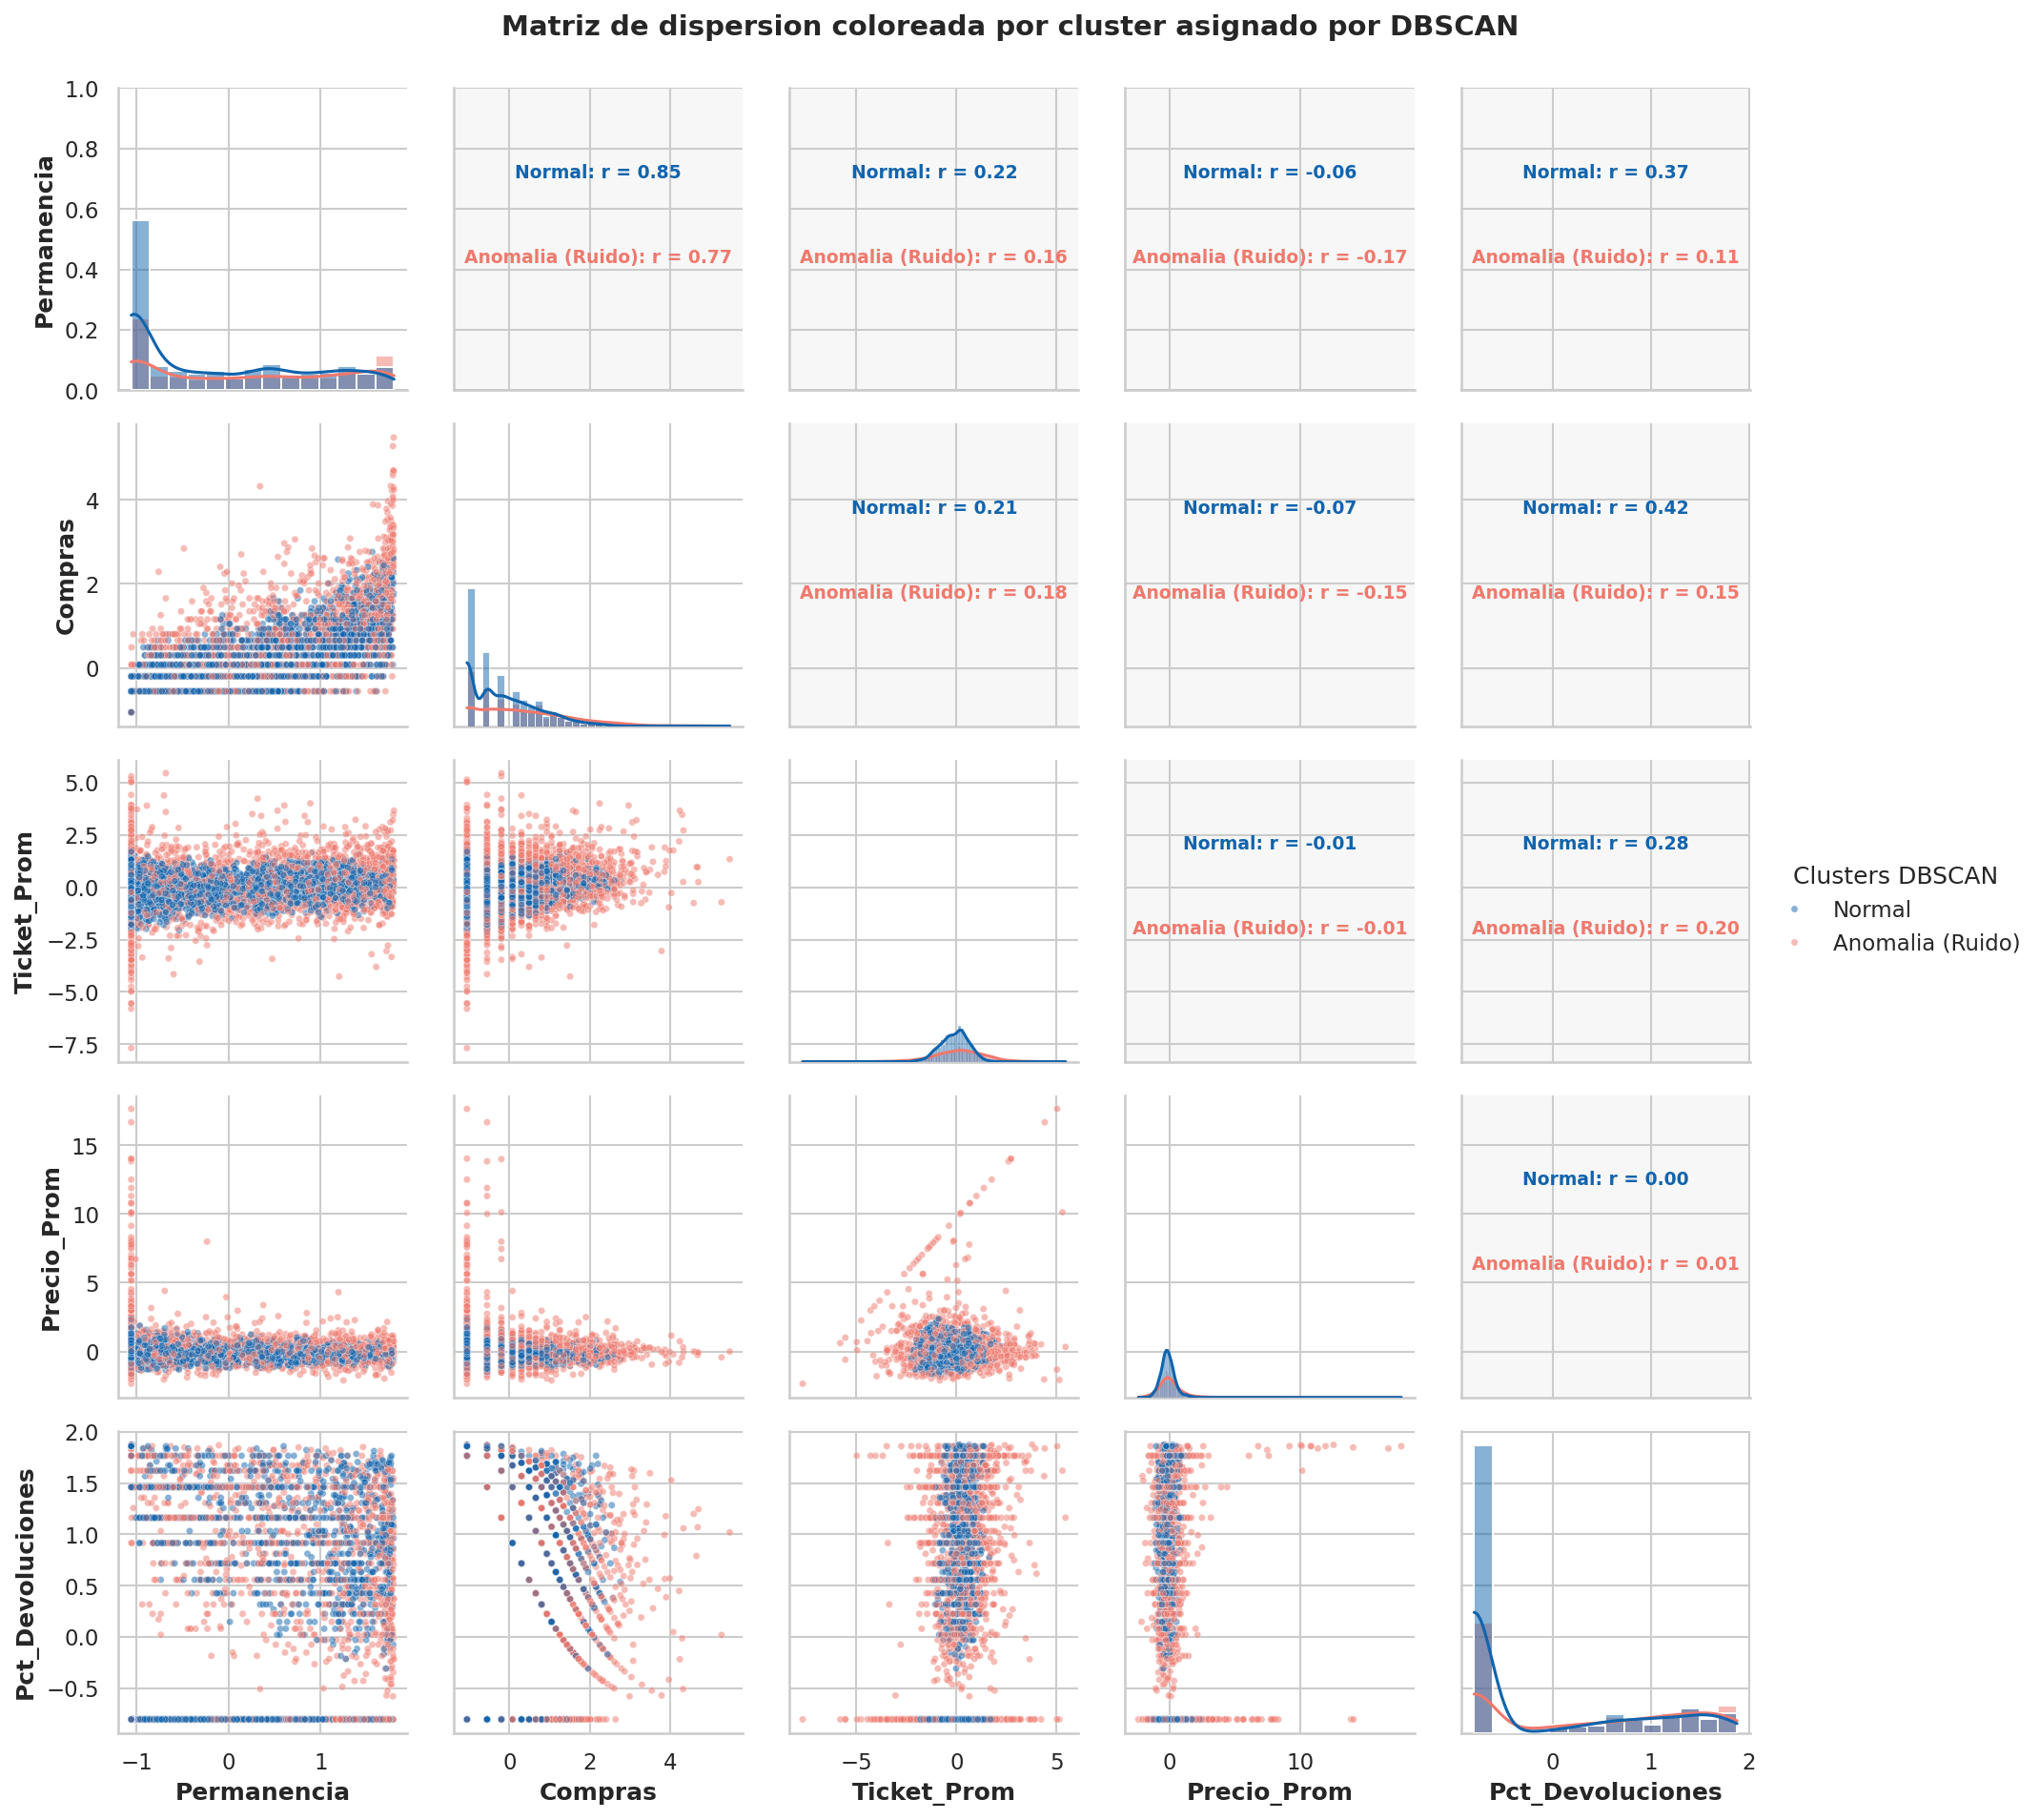
\includegraphics[width=0.85\textwidth]{fig05_dispersion_cluster_dbscan.png}
    \caption{Matriz de dispersión de variables seleccionadas (Permanencia, Compras, Ticket\_Prom, Precio\_Prom, Pct\_Devoluciones), coloreada según la etiqueta binaria de anomalía asignada por DBSCAN (Normal vs.\ Anomalía/Ruido), con la correlación de Pearson de cada grupo anotada en el triángulo superior.}
    \label{fig:dispersion-dbscan}
\end{figure}

\begin{figure}[H]
    \centering
    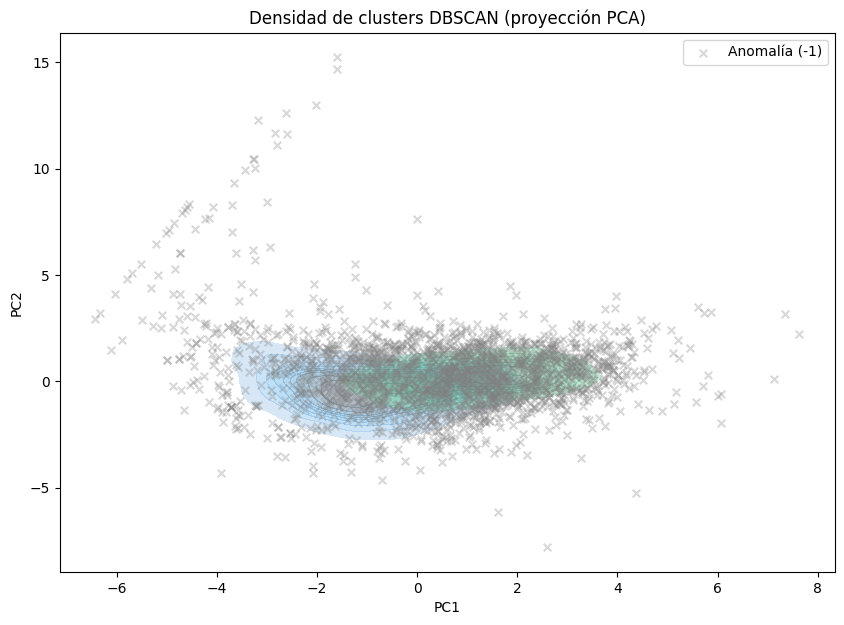
\includegraphics[width=0.7\textwidth]{fig06_densidad_dbscan_pca.png}
    \caption{Densidad de los clusters de DBSCAN sobre la proyección PCA (2 componentes).}
    \label{fig:densidad-dbscan}
\end{figure}

El gráfico de densidad muestra un único núcleo denso central (correspondiente a los dos clusters reales)
rodeado de una nube dispersa y extensa de puntos de ruido.

\subsection*{Isolation Forest}

Isolation Forest aborda la detección de anomalías desde un principio distinto al de los modelos basados
en distancia o densidad: en lugar de modelar qué es ``normal'' y señalar lo que no encaja, modela
directamente qué tan fácil es aislar una observación del resto mediante particiones aleatorias del espacio
de variables.

El modelo construye un ensamble de árboles de aislamiento (\textit{isolation trees}). Cada árbol se construye de
forma recursiva: en cada nodo se selecciona al azar una variable y, dentro de su rango de valores presente
en ese nodo, un punto de corte aleatorio, dividiendo las observaciones en dos ramas. Este proceso se
repite hasta que cada observación queda aislada en su propio nodo hoja, o se alcanza una profundidad
máxima.

El score de anomalía de una observación $x$ se define como:

\begin{equation}
s(x, n) = 2^{-E[h(x)] / c(n)}
\end{equation}

Este score se interpreta de la siguiente manera:

\begin{itemize}
    \item $s(x,n)$ cercano a 1: longitud de camino muy corta. Observación con alta probabilidad de ser anómala.
    \item $s(x,n)$ cercano a 0.5: longitud de camino cercana al promedio esperado. Observación normal.
    \item $s(x,n)$ considerablemente menor a 0.5: la observación requirió muchos cortes para aislarse. Comportamiento muy típico.
\end{itemize}

\subsubsection*{Optimización de hiperparámetros}

Al igual que con DBSCAN, no existe una variable objetivo contra la cual validar el modelo, por lo que se
mantuvo el mismo criterio de optimización (Silhouette Score sobre las etiquetas $-1/1$ producidas por el
modelo) para conservar consistencia metodológica entre ambos modelos y permitir una comparación
bajo el mismo criterio. Se utilizó nuevamente Optuna con TPE, optimizando 20 iteraciones sobre los
siguientes hiperparámetros:

\begin{itemize}
    \item \textbf{n\_estimators:} número de árboles de aislamiento en el ensamble [50, 300].
    \item \textbf{max\_samples:} fracción de observaciones utilizada para construir cada árbol [0.1, 1.0].
    \item \textbf{contamination:} proporción esperada de anomalías en el dataset, usada para fijar el umbral de decisión.
    \item \textbf{max\_features:} fracción de variables consideradas en cada partición.
\end{itemize}

\begin{table}[H]
\centering
\begin{tabular}{ll}
\toprule
\textbf{Hiperparámetro} & \textbf{Valor óptimo} \\
\midrule
n\_estimators & 236 \\
max\_samples & 0.5739 \\
contamination & 0.0133 \\
max\_features & 0.9840 \\
\bottomrule
\end{tabular}
\caption{Hiperparámetros óptimos de Isolation Forest.}
\end{table}

El mejor Silhouette Score obtenido fue de 0.5835, considerablemente superior al de DBSCAN (0.0805).

\subsubsection*{Resultados del modelo}

Con los hiperparámetros óptimos, Isolation Forest marcó 79 clientes (1.34\% del total) como anómalos, un
porcentaje mucho más acotado que el 39.06\% de DBSCAN, y más cercano a lo que intuitivamente se
esperaría de un conjunto de ``casos atípicos'' dentro de una base de clientes.

\begin{figure}[H]
    \centering
    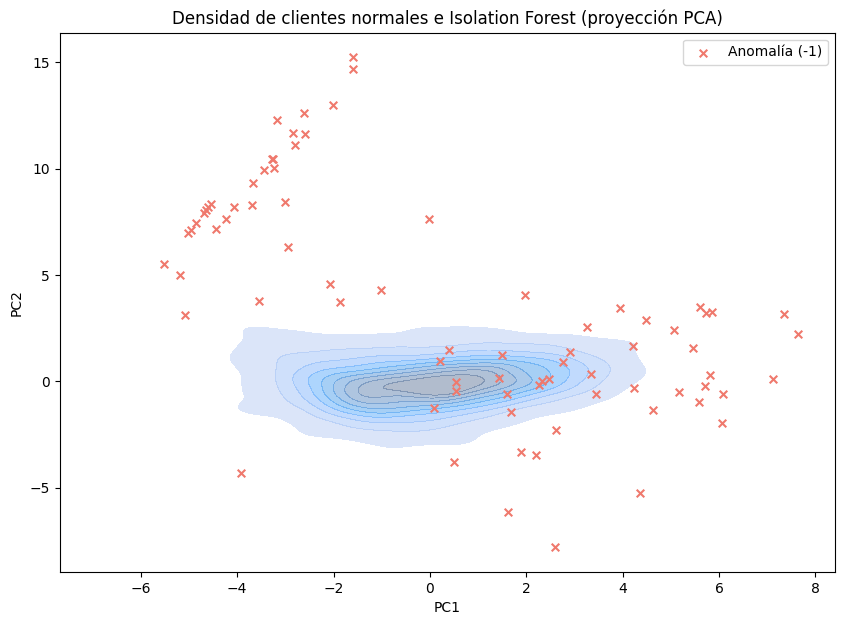
\includegraphics[width=0.7\textwidth]{fig07_densidad_isof_pca.png}
    \caption{Densidad de los puntos normales y anomalías de Isolation Forest.}
    \label{fig:densidad-isof}
\end{figure}

A diferencia del gráfico de DBSCAN, aquí las anomalías no forman una nube dispersa que rodea todo el
núcleo denso, sino que se concentran en un subconjunto más acotado de posiciones.

\section*{Evaluación de Resultados}
\addcontentsline{toc}{section}{Evaluación de Resultados}

\subsection*{Métricas de evaluación para modelos no supervisados}

Al no existir etiquetas de verdad conocida (\textit{ground truth}) sobre qué clientes son realmente anómalos, la
evaluación de ambos modelos se apoyó en tres tipos de evidencia complementaria:

\begin{itemize}
    \item una métrica interna de calidad de agrupamiento (Silhouette Score),
    \item el porcentaje de observaciones marcadas como anomalía (relevancia práctica para el negocio), y
    \item el perfil estadístico de las anomalías detectadas frente a los clientes normales (validación cualitativa de que el patrón detectado tiene sentido).
\end{itemize}

\subsection*{Evaluación de DBSCAN}

Los resultados obtenidos fueron los siguientes:

\begin{table}[H]
\centering
\begin{tabular}{ll}
\toprule
Silhouette Score & 0.08053290539470856 \\
Anomalías detectadas por DBSCAN & 2295 \\
Porcentaje & 39.0571817562968 \% \\
\bottomrule
\end{tabular}
\end{table}

\begin{figure}[H]
    \centering
    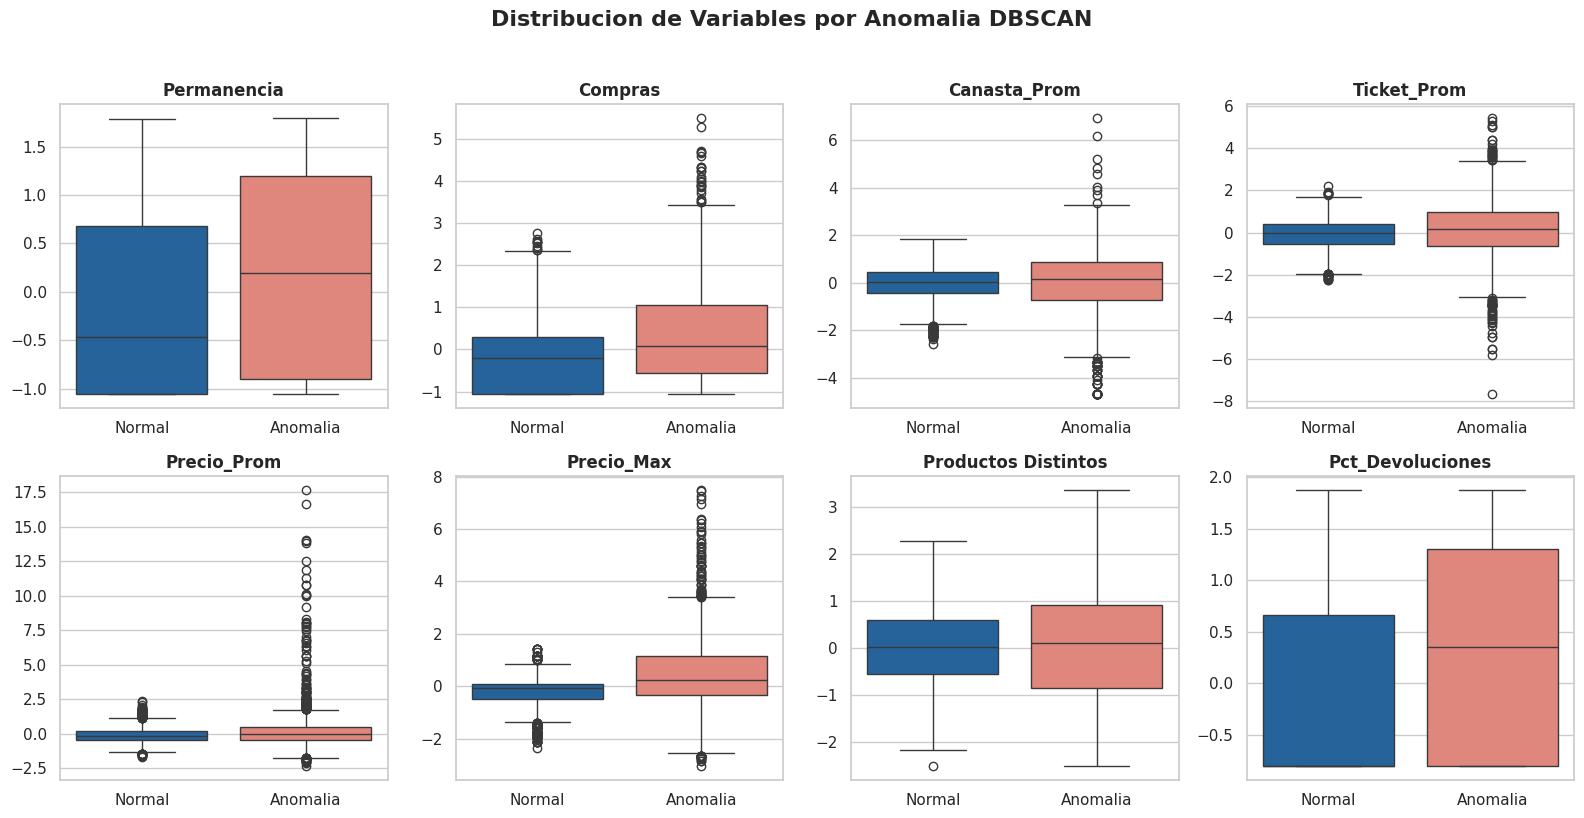
\includegraphics[width=0.85\textwidth]{fig08_boxplots_anomalia_dbscan.png}
    \caption{Distribución de cada variable, comparando clientes normales contra los marcados como anomalía (ruido) por DBSCAN.}
    \label{fig:boxplots-dbscan}
\end{figure}

\begin{table}[H]
\centering
\begin{tabular}{lccccc}
\toprule
\textbf{Grupo} & \textbf{Permanencia} & \textbf{Compras} & \textbf{Ticket\_Prom} & \textbf{Precio\_Max} & \textbf{Pct\_Devoluciones} \\
\midrule
Normal (0) & -0.13 & -0.20 & -0.09 & -0.22 & -0.19 \\
Anomalía (1) & 0.21 & 0.31 & 0.14 & 0.34 & 0.30 \\
\bottomrule
\end{tabular}
\caption{Valores promedio (en unidades estandarizadas) de una selección de variables por grupo.}
\end{table}

\begin{itemize}
    \item \textbf{Silhouette Score:} el valor obtenido (0.08) está muy cerca de 0, lo que indica que los clusters formados por DBSCAN se encuentran considerablemente solapados entre sí.
    \item \textbf{Porcentaje de anomalías:} DBSCAN marcó como ruido al 39.06\% de los clientes. Este porcentaje es demasiado alto para considerarse un conjunto de anomalías accionable desde el punto de vista de negocio; refleja más bien zonas de baja densidad del espacio de variables que el algoritmo no logra asignar a ninguno de los 2 clusters encontrados.
    \item \textbf{Perfil promedio:} los clientes marcados como anomalía muestran valores ligeramente más altos en Permanencia, Compras, Ticket\_Prom, Precio\_Max y Pct\_Devoluciones, pero las diferencias frente a los clientes normales son pequeñas (menores a 0.35 desviaciones estándar). Esto refuerza que el ``ruido'' de DBSCAN no corresponde a un grupo de outliers extremos, sino a clientes en zonas de transición entre clusters.
    \item \textbf{Conclusión parcial:} DBSCAN logra segmentar un cluster mayoritario de clientes con comportamiento típico, pero su definición de anomalía (el ruido) resulta demasiado amplia y poco discriminativa para usarse como detección de anomalías por sí sola.
\end{itemize}

\subsection*{Evaluación de Isolation Forest}

\begin{figure}[H]
    \centering
    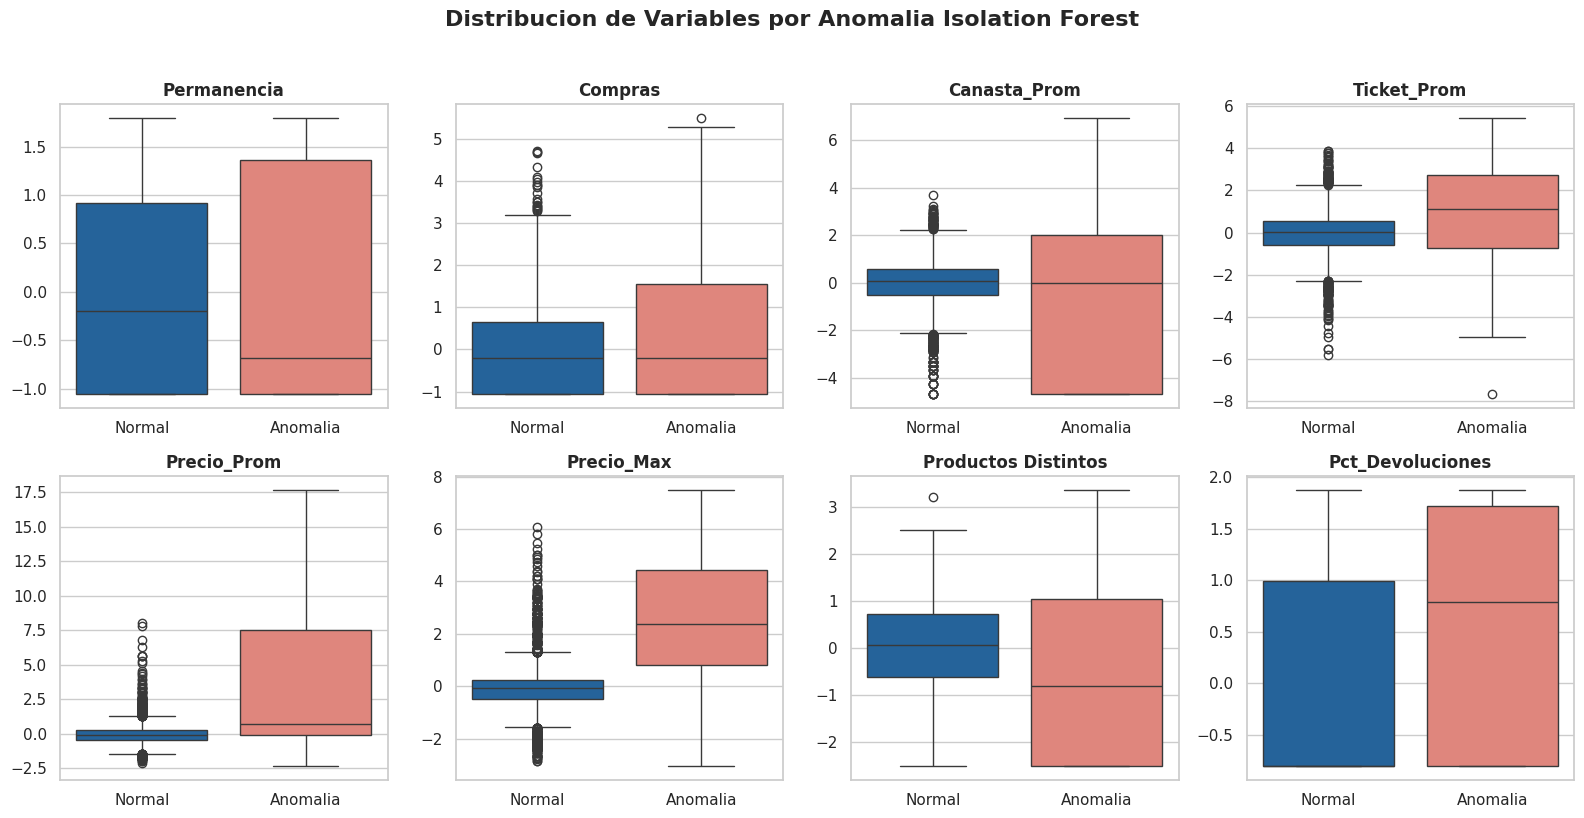
\includegraphics[width=0.85\textwidth]{fig09_boxplots_anomalia_isof.png}
    \caption{Distribución de cada variable, comparando clientes normales contra los marcados como anomalía por Isolation Forest.}
    \label{fig:boxplots-isof}
\end{figure}

\begin{table}[H]
\centering
\begin{tabular}{lccccc}
\toprule
\textbf{Grupo} & \textbf{Compras} & \textbf{Ticket\_Prom} & \textbf{Precio\_Prom} & \textbf{Precio\_Max} & \textbf{Pct\_Devoluciones} \\
\midrule
Normal (0) & -0.01 & -0.01 & -0.05 & -0.03 & -0.01 \\
Anomalía (1) & 0.54 & 0.91 & 3.46 & 2.52 & 0.54 \\
\bottomrule
\end{tabular}
\caption{Valores promedio (en unidades estandarizadas) de una selección de variables por grupo.}
\end{table}

\begin{itemize}
    \item \textbf{Silhouette Score:} el valor obtenido ($\sim$0.58) es considerablemente más alto que el de DBSCAN ($\sim$0.08), lo que indica que el grupo de anomalías identificado por Isolation Forest está mucho mejor separado del resto de los clientes.
    \item \textbf{Porcentaje de anomalías:} Isolation Forest marcó únicamente al 1.34\% de los clientes (79 de 5,876) como anomalía, un porcentaje mucho más razonable y accionable para el negocio que el 39.06\% de DBSCAN.
    \item \textbf{Perfil promedio:} a diferencia de DBSCAN, los clientes anómalos de Isolation Forest muestran diferencias marcadas frente a los normales, sobre todo en Precio\_Prom (+3.46 desviaciones estándar) y Precio\_Max (+2.52), además de Ticket\_Prom (+0.91) y Pct\_Devoluciones (+0.54). Esto describe un grupo de clientes que compra productos considerablemente más caros de lo usual y/o que tiene tasas de devolución elevadas.
    \item \textbf{Conclusión parcial:} Isolation Forest logra aislar un grupo pequeño y bien diferenciado de clientes atípicos, en lugar de simplemente etiquetar como ruido a los clientes en zonas de baja densidad, lo que lo hace más adecuado que DBSCAN para esta tarea específica.
\end{itemize}

\subsection*{Comparación entre modelos}

\begin{figure}[H]
    \centering
    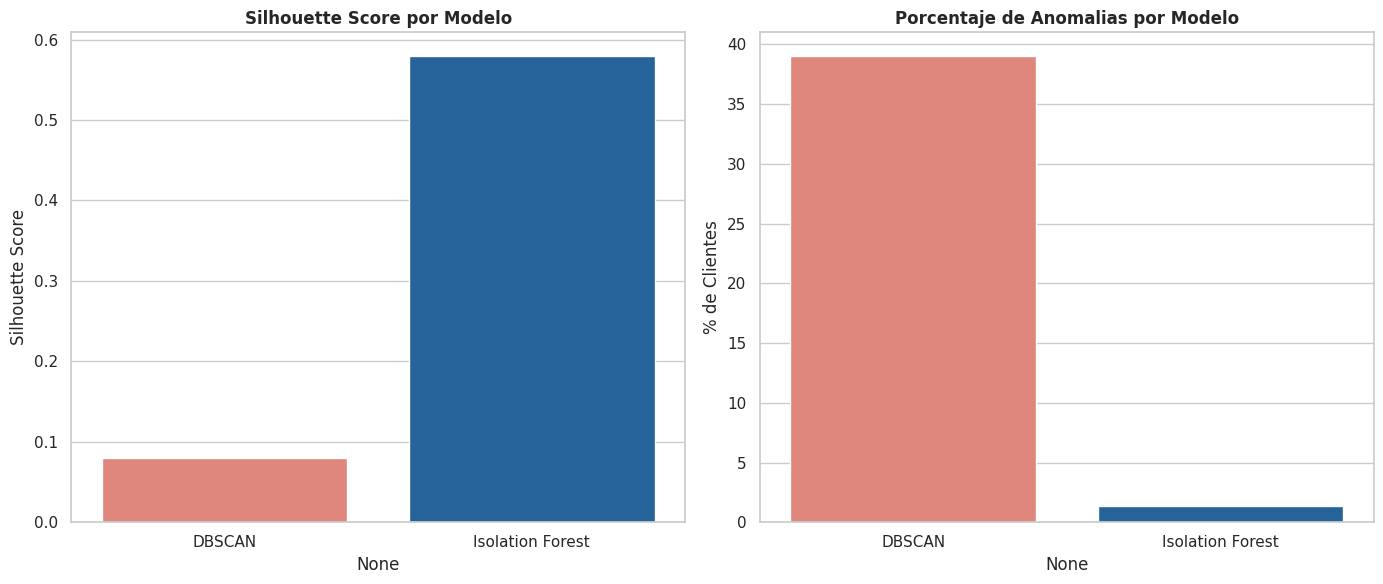
\includegraphics[width=0.85\textwidth]{fig10_comparacion_modelos.png}
    \caption{Comparación de Silhouette Score y porcentaje de anomalías detectadas entre ambos modelos.}
    \label{fig:comparacion}
\end{figure}

\begin{table}[H]
\centering
\begin{tabular}{lccc}
\toprule
\textbf{Modelo} & \textbf{Silhouette Score} & \textbf{Anomalías detectadas} & \textbf{\% del total} \\
\midrule
DBSCAN & 0.08 & 2,295 & 39.06\% \\
Isolation Forest & 0.58 & 79 & 1.34\% \\
\bottomrule
\end{tabular}
\end{table}

\subsubsection*{Tabla cruzada: coincidencia entre modelos}

\begin{table}[H]
\centering
\begin{tabular}{lcc}
\toprule
\textbf{DBSCAN $\backslash$ Isolation Forest} & \textbf{Anomalía} & \textbf{Normal} \\
\midrule
Anomalía & 79 & 2,216 \\
Normal & 0 & 3,581 \\
\bottomrule
\end{tabular}
\end{table}

\textbf{Coincidencia entre modelos:} la tabla cruzada muestra que las 79 anomalías detectadas por Isolation Forest
son un subconjunto de los clientes que DBSCAN ya marcaba como ruido. Esto sugiere que Isolation Forest
logra aislar, dentro del amplio grupo de ruido de DBSCAN, a los casos verdaderamente extremos. Un
porcentaje de anomalías tan alto como el de DBSCAN (39.06\%) es poco útil para el negocio, ya que no
permite priorizar acciones sobre un grupo reducido y manejable de clientes.

\section*{Conclusión}
\addcontentsline{toc}{section}{Conclusión}

Dado el objetivo de detección de clientes anómalos sobre este conjunto de datos, \textbf{Isolation Forest resultó
ser el modelo más adecuado}. Obtuvo un Silhouette Score considerablemente mayor (0.58 frente a 0.08),
identificó un porcentaje de anomalías mucho más razonable, y su perfil resultó mucho más interpretable
y susceptible de traducirse en una acción comercial concreta.

DBSCAN, por su parte, resultó más útil como herramienta de segmentación general (encontró un cluster
mayoritario coherente de clientes con comportamiento típico) que como detector de anomalías por sí
solo, dado que su noción de ``ruido'' terminó siendo demasiado amplia y poco discriminativa para este
dataset en particular, donde el comportamiento de compra se distribuye como un continuo más que como
grupos de densidad claramente separados.

La elección entre un modelo basado en densidad y uno basado en aislamiento depende de la estructura
real de los datos. Cuando las observaciones no forman clusters de densidad bien delimitados, reutilizar el
``ruido'' de un algoritmo de clustering como proxy de anomalía puede sobreestimar considerablemente el
tamaño del grupo atípico, mientras que un modelo diseñado específicamente para aislamiento
estructural, como Isolation Forest, tiende a producir un conjunto de anomalías más acotado y accionable.

\section*{Referencias}
\addcontentsline{toc}{section}{Referencias}

\begin{itemize}
    \item Chen, D. (2015). \textit{Online Retail} [Dataset]. UCI Machine Learning Repository. \url{https://doi.org/10.24432/C5BW33}
    \item Optuna. (n.d.). \textit{Optuna: A hyperparameter optimization framework}. Retrieved August 9, 2026, from \url{https://optuna.org/}
    \item Scikit-learn. (n.d.). \textit{sklearn.ensemble.IsolationForest}. Retrieved August 9, 2026, from \url{https://scikit-learn.org/stable/modules/generated/sklearn.ensemble.IsolationForest.html}
    \item Scikit-learn. (n.d.). \textit{sklearn.cluster.DBSCAN}. Retrieved August 9, 2026, from \url{https://scikit-learn.org/stable/modules/generated/sklearn.cluster.DBSCAN.html}
\end{itemize}

\end{document}
